\documentclass[12pt,a4paper]{article}
\usepackage[T1]{fontenc}
\usepackage{amsmath,amssymb,mathrsfs,tikz,times,pifont}
\usepackage{enumitem}
\usetikzlibrary{trees}
\newcommand\circitem[1]{%
\tikz[baseline=(char.base)]{
\node[circle,draw=gray, fill=red!55,
minimum size=1.2em,inner sep=0] (char) {#1};}}
\newcommand\boxitem[1]{%
\tikz[baseline=(char.base)]{
\node[fill=cyan,
minimum size=1.2em,inner sep=0] (char) {#1};}}
\setlist[enumerate,1]{label=\protect\circitem{\arabic*}}
%%%::::::by chnini ameur :::::::%%%
\everymath{\displaystyle}
\usepackage[left=1cm,right=1cm,top=1cm,bottom=1.7cm]{geometry}
\usepackage[colorlinks=true, linkcolor=blue, urlcolor=blue, citecolor=blue]{hyperref}
\usepackage{array,multirow}
\usepackage[most]{tcolorbox}
\usepackage{varwidth}
\usepackage{float} %pour utiliser l'option [H] qui force l'image à apparaître exactement à l'endroit où elle est placée dans le code.
\tcbuselibrary{skins,hooks}
\usetikzlibrary{patterns}
%%%::::::by chnini ameur :::::::%%%
\newtcolorbox{exa}[2][]{enhanced,breakable,before skip=2mm,after skip=5mm,
colback=yellow!20!white,colframe=black!20!blue,boxrule=0.5mm,
attach boxed title to top left ={xshift=0.6cm,yshift*=1mm-\tcboxedtitleheight},
fonttitle=\bfseries,
title={#2},#1,
% varwidth boxed title*=-3cm,
boxed title style={frame code={
\path[fill=tcbcolback!30!black]
([yshift=-1mm,xshift=-1mm]frame.north west)
arc[start angle=0,end angle=180,radius=1mm]
([yshift=-1mm,xshift=1mm]frame.north east)
arc[start angle=180,end angle=0,radius=1mm];
\path[left color=tcbcolback!60!black,right color = tcbcolback!60!black,
middle color = tcbcolback!80!black]
([xshift=-2mm]frame.north west) -- ([xshift=2mm]frame.north east)
[rounded corners=1mm]-- ([xshift=1mm,yshift=-1mm]frame.north east)
-- (frame.south east) -- (frame.south west)
-- ([xshift=-1mm,yshift=-1mm]frame.north west)
[sharp corners]-- cycle;
},interior engine=empty,
},interior style={top color=yellow!5}}
%%%%%%%%%%%%%%%%%%%%%%%
% Création du compteur pour les exercices
\newcounter{exercice}
\renewcommand{\theexercice}{\arabic{exercice}}  % Définit l'affichage du compteur en chiffres arabes

% Définir la commande \exo
\newcommand{\exo}{\refstepcounter{exercice}\textbf{Exercice \theexercice} }

\usepackage{fancyhdr}
\usepackage{eso-pic}         % Pour ajouter des éléments en arrière-plan
% Commande pour ajouter du texte en arrière-plan
\usepackage{tkz-tab}
\AddToShipoutPicture{
    \AtTextCenter{%
        \makebox[0pt]{\rotatebox{80}{\textcolor[gray]{0.7}{\fontsize{5cm}{5cm}\selectfont PGB}}}
    }
}
\usepackage{lastpage}
\fancyhf{}
\pagestyle{fancy}
\renewcommand{\footrulewidth}{1pt}
\renewcommand{\headrulewidth}{0pt}
\renewcommand{\footruleskip}{10pt}
\fancyfoot[R]{
\color{blue}\ding{45}\ \textbf{2025}
}
\fancyfoot[L]{
\color{blue}\ding{45}\ \textbf{Prof:M. BA}
}
\cfoot{\bf
\thepage /
\pageref{LastPage}}
\begin{document}
\renewcommand{\arraystretch}{1.5}
\renewcommand{\arrayrulewidth}{1.2pt}
\begin{tikzpicture}[overlay,remember picture]
    \node[draw=blue,line width=1.2pt,fill=purple,text=blue,inner sep=3mm,rounded corners,pattern=dots]at ([yshift=-2.5cm]current page.north) {\begingroup\setlength{\fboxsep}{0pt}\colorbox{white}{\begin{tabular}{|*1{>{\centering \arraybackslash}p{0.28\textwidth}} |*2{>{\centering \arraybackslash}p{0.2\textwidth}|} *1{>{\centering \arraybackslash}p{0.19\textwidth}|} }
                \hline
                \multicolumn{3}{|c|}{$\diamond$$\diamond$$\diamond$\ \textbf{Lycée de Dindéfélo}\ $\diamond$$\diamond$$\diamond$ } & \textbf{A.S. : 2024/2025}                                              \\ \hline
                \textbf{Matière: Mathématiques}                                                                                    & \textbf{Niveau : T}\textbf{S2} & \textbf{Date: 17/04/2025} & \textbf{} \\ \hline
                \multicolumn{4}{|c|}{\parbox[c]{10cm}{\begin{center}
                                                                  \textbf{{\Large\sffamily Td Probabilité}}
                                                              \end{center}}}                                                                                                        \\ \hline
            \end{tabular}}\endgroup};
\end{tikzpicture}
\vspace{3cm}

\section*{\fbox{\textbf{\exo}}}

Un jeu de 32 cartes est constitué de 4 couleurs : Piques, coeur, trèfle et carreau. Chaque couleur est composé de 8 cartes : l'As ; le Roi, la Dame, le Valet, le 10, le 9, le 8 et le 7.

\begin{enumerate}
    \item On tire simultanément 3 cartes de ce jeu. Calculer la probabilité de chacun des événements suivants :
    \begin{enumerate}
        \item $A :$ "Les trois cartes sont des As"
        \item $B :$ "Il y a au moins deux couleurs parmi les trois cartes"
        \item $C :$ "Il n'y a pas d'As parmi les trois cartes"
    \end{enumerate}
    \item On tire successivement avec remise 3 cartes du jeu de 32 cartes. On définit la variable aléatoire $X$ qui est égale au nombre de couleurs tiré. Déterminer la loi de probabilité de $X$.
\end{enumerate}

\section*{\fbox{\textbf{\exo}}}

Une urne contient 12 fiches portant chacune une lettre du mot "BACCALAUREAT".

\begin{enumerate}
    \item On tire successivement et au hasard les 12 fiches en les plaçant l'une après l'autre. Quelle est la probabilité d'obtenir :
    \begin{enumerate}
        \item Un mot commençant par une consonne ?
        \item Un mot commençant par une voyelle ?
        \item Le mot BACCALAUREAT ?
    \end{enumerate}
    \item On remet les fiches dans l'urne et on en tire que 3 fiches toujours successivement et sans remise. Quelle est la probabilité d'obtenir :
    \begin{enumerate}
        \item Le mot BAC.
        \item Trois voyelles.
        \item Un seul A.
        \item Au moins un A.
    \end{enumerate}
\end{enumerate}

\section*{\fbox{\textbf{\exo}}}

Les laboratoires pharmaceutiques indiquent pour chaque test sa sensibilité $\alpha$, qui est la probabilité que le test soit positif si le sujet est malade, et sa spécificité $\beta$, qui est la probabilité que le test soit négatif si le sujet est sain. Sachant qu'en moyenne il y a un malade sur 1000 personnes, calculer la probabilité d’être un sujet sain alors que le test est positif, avec $\alpha = 95\%$ et $\beta = 97\%$. Calculer la probabilité d’être malade alors que le test est négatif.

\section*{\fbox{\textbf{\exo}}}

Une porte monnaie comprend quatre pièces de 500F et six pièces de 200F. Un enfant tire au hasard simultanément 3 pièces de ce porte monnaie.

\begin{enumerate}
    \item Calculer la probabilité de l’événement $A$ : ``tirer 3 pièces de 500F''.
    \item Soit $X$ la variable aléatoire égale au nombre de pièces de 500F tiré.
    \begin{enumerate}
        \item Déterminer la loi de probabilité de $X$.
        \item Calculer l’espérance mathématique de $X$ et son écart type.
    \end{enumerate}
    \item L’enfant répète 5 fois la même épreuve en remettant à chaque fois les trois pièces tirées dans le porte monnaie. Quelle est la probabilité que l’événement $A$ se réalise trois fois à l’issue de l’épreuve ?
\end{enumerate}

\section*{\fbox{\textbf{\exo}}}

Une urne contient neuf boules : trois rouges numérotées $-1$, $-1$, $1$, deux vertes numérotées $-2$, $2$ et quatre blanches numérotées $1$, $-2$, $2$, $2$. Toutes les boules sont indiscernables au toucher.
\begin{enumerate}
    \item  On tire \textbf{simultanément trois boules} de l’urne. Calculer la probabilité des événements suivants :
          \begin{itemize}
              \item[$A$] "avoir trois boules de même couleur"
              \item[$B$] "avoir trois boules dont le produit des numéros marqués est négatif"
              \item[$C$] "avoir trois boules de même couleur et de produit négatif"
              \item[$D$] "avoir trois boules de produit négatif \textbf{ou} de même couleur"
          \end{itemize}
    \item On tire \textbf{3 boules successivement et avec remise}. Calculer la probabilité des événements suivants :
          \begin{itemize}
              \item[$E$] "Avoir trois boules de couleurs différentes"
              \item[$F$] "avoir trois boules de couleurs différentes dont le premier est rouge"
          \end{itemize}
\end{enumerate}

\section*{\fbox{\textbf{\exo}}}

On dispose de deux dés cubiques parfaits $A$ et $B$. Les faces du dé $A$ sont numérotées $0,1,1,-1,-1,-1$ et celles du dé $B$ sont numérotées $0,0,0,1,1,1$.
\begin{enumerate}
    \item On lance les deux dés. À chaque lancer, on construit un nombre complexe $z = a + ib$ où $a$ est le numéro obtenu du dé $A$ et $b$ le numéro obtenu du dé $B$.\\
          Calculer la probabilité des événements suivants :
          \begin{itemize}
              \item[$A$] "$z = 0$"
              \item[$B$] "$z$ est réel"
              \item[$C$] "$z$ est imaginaire pur non nul"
              \item[$D$] "$|Z| = \sqrt{2}$"
              \item[$E$] "$\Re(z) > 0$"
              \item[$F$] "$D \cup E$"
          \end{itemize}

    \item  On lance le dé $A$ quatre fois de suite.
          \begin{enumerate}
              \item Calculer la probabilité pour que la somme des numéros obtenus soit nulle.
              \item Calculer la probabilité pour que le produit des numéros obtenus soit nul.
          \end{enumerate}
\end{enumerate}

\section*{\fbox{\textbf{\exo}}}

Une usine fabrique en grande série de climatiseurs susceptibles de présenter deux défauts $a$ et $b$. Une étude statistique de la production conduit aux résultats suivants :
\begin{itemize}
    \item 7\% des climatiseurs présentent le défaut $a$.
    \item Parmi les climatiseurs présentant le défaut $a$, 9\% présentent le défaut $b$.
    \item Parmi les climatiseurs ne présentant pas le défaut $a$, 6\% présentent le défaut $b$.
\end{itemize}
On prélève au hasard un climatiseur de la production. On désigne par $A$ et $B$ les événements suivants :

$A$ « le climatiseur présente le défaut $a$ » et $B$ « le climatiseur présente le défaut $b$ ».

\begin{tikzpicture}[level distance=3cm,
        level 1/.style={sibling distance=5cm},%Ecarte les branches des 1eme ramifications
        level 2/.style={sibling distance=4cm},%Ecarte les branches des  2eme ramifications
        %level 3/.style={sibling distance=2cm}]%Ecarte les branches des 3eme ramifications
        every node/.style={text width=2cm, align=center}]%Permet de spécifier une largeur pour chaque nœud
    \node {}
    child {node {$\overline{A}$}
            child {node {$\overline{B}$}
                }
            child {node {$B$}
                }
        }% 1ere branche      
    child {node {$A$}
            child {node {$\overline{B}$}
                }
            child {node {$B$}
                }
        };
    %\node at (-3,-1.5) [right] {$1$};

    \node at (0.8,-1.5) [right] {};

    \node at (0.8,-1.5) [right] {$0.07$};

    %\node at (-5,-4) [right] {$0,90$};
    \node at (-2.5,-4) [right] {$0,06$};

    %\node at (-0.1,-4) [right] {$0,90$};
    \node at (2.5,-4) [right] {$0,09$};
\end{tikzpicture}

\begin{enumerate}
    \item L’arbre pondéré ci-contre représente cette situation. Recopier et compléter cet arbre.
    \item
          \begin{enumerate}
              \item Calculer $p(A \cap B)$.
              \item Montrer que $p(B) = 0.0621$.
              \item Quelle est la probabilité que le climatiseur ne présente aucun défaut
          \end{enumerate}
    \item Sachant que le climatiseur présente le défaut $b$, quelle est la probabilité que ce climatiseur présente le défaut $a$.
\end{enumerate}

\section*{\fbox{\textbf{\exo}}\quad BAC S2 2003}

Dans un pays donné, la maladie du sida touche cinq pour mille de sa population.

Des études statistiques montrent que la probabilité pour un individu d’avoir un test positif à cette maladie sachant qu’il est malade
est 0,8 et celui d’avoir un test négatif sachant qu’il n"est pas atteint par la maladie est 0,9.
On note : $T$ l’événement « avoir un test positif à cette maladie »

$M$ l’événement « être malade »

$\overline{M}$ est l’événement contraire de $M$.

On rappelle que pour tous événements $A$ et $B$, on a :

$A = (A \cap B) \cup (A \cap \overline{B}) \quad \text{et} \quad P_A(B) \text{ désigne la probabilité de } B \text{ sachant } A.$

\begin{enumerate}
    \item
          \begin{enumerate}
              \item Réécrire la relation $(*)$ pour $A = T$ et $B = M$, puis pour $A = \overline{M}$ et $B = \overline{T}$.
              \item En déduire que $P(A \cap \overline{M}) = P(\overline{M}) \left[ 1 - P_{\overline{M}}(\overline{T}) \right]$
              \item Calculer la probabilité pour qu’un individu ait un test positif à cette maladie.
          \end{enumerate}
    \item
          \begin{enumerate}
              \item Calculer la probabilité pour qu’un individu soit malade sachant qu’il a un test positif à cette maladie.
              \item Calculer la probabilité pour qu’un individu soit malade sachant qu’il a un test négatif à cette maladie.
          \end{enumerate}
          On donnera les résultats sous forme de fraction irréductible.
\end{enumerate}

\section*{\fbox{\textbf{\exo}}}

Soit un dé cubique dont les faces sont numérotées de 1 à 6. Lorsqu’on lance ce dé, on note par $p_i$ la probabilité d’apparition de la face numérotée $i$ ($i = 1, 2, 3, 4, 5, 6$).
\begin{itemize}
    \item $p_1, p_3$ et $p_5$ sont dans cet ordre en progression géométrique de raison $\frac{1}{2}$.
    \item $p_2, p_4$ et $p_6$ sont dans cet ordre en progression arithmétique de raison $\frac{1}{8}$ et $2p_2 = 3p_1$.
\end{itemize}

\begin{enumerate}
    \item Déterminer $p_1, p_2, p_3, p_4, p_5$ et $p_6$.
    \item On lance ce dé 4 fois de suite et on note $X$ la variable aléatoire égale au nombre de fois qu’on obtient un nombre pair au cours des 4 lancers.
          \begin{enumerate}
              \item Déterminer la loi de probabilité de $X$.
              \item Déterminer $E(X)$ et $\sigma(X)$.
              \item Déterminer la fonction de répartition de $X$.
          \end{enumerate}
    \item Cette fois-ci on lance $n$ fois de suite. Déterminer le plus petit entier naturel $n$ pour que la probabilité d’avoir au moins une fois un numéro pair soit supérieur ou égal à 0,99.
\end{enumerate}

\section*{\fbox{\textbf{\exo}}}

On dispose d’un dé cubique dont les faces sont numérotées de 1 à 6. On désigne par $p_i$ la probabilité d’apparition de la face $i$ lors d’un lancer du dé. Le dé est pipé de telle manière que $p_1, p_2, p_3, p_4, p_5$ et $p_6$ sont dans cet ordre six termes consécutifs d’une suite géométrique de raison $q = \frac{1}{2}$.
\begin{enumerate}
    \item Montrer que $p_1 = \frac{32}{63}$ puis en déduire $p_2, p_3, p_4, p_5$ et $p_6$.
    \item Soit $A$ l’événement « obtenir un chiffre pair », montrer que $p(A) = \frac{1}{3}$.
    \item On dispose maintenant d’une urne $U$ contenant
          \begin{itemize}
              \item si $A$ est réalisé alors on tire successivement et sans remise deux jetons de $U$.
              \item sinon on tire simultanément deux jetons de $U$.
          \end{itemize}
          Soit $D$ l’événement « les deux jetons tirés sont de couleurs différentes ».
          \begin{enumerate}
              \item Calculer $p(D \cap A)$ et $p(D \cap \overline{A})$.
              \item En déduire que $p(D) = \frac{3}{5}$ puis calculer $p_{D}(A)$.
          \end{enumerate}
    \item On répète 10 fois de suite dans les mêmes conditions et de façon indépendantes le tirage précédent. Soit $X$ la variable aléatoire égale aux nombres de réalisations de l’événement $D$ à l’issu des deux tirages.
          \begin{enumerate}
              \item Déterminer la probabilité d’avoir exactement deux fois l’événement $D$.
              \item Déterminer la probabilité d’avoir au moins une fois l’événement $D$ à l’issu des 10 tirages.
              \item Calculer l’espérance mathématique et l’écart type de $X$.
          \end{enumerate}
\end{enumerate}

\section*{\fbox{\textbf{\exo}}\quad BAC S2 2011}

\textbf{I.} On considère $\Omega$ l'univers associé à une expérience aléatoire, $A$ et $B$ deux événements. Dans le cas d’équiprobabilité rappeler les probabilités des événements suivants :

\textbf{$A$, $A$ sachant $B$}, $A \cap B$, $(A \cap B) \cup (A \cap \overline{B})$.

\textbf{II.} Une société de distribution d’électricité ayant une production insuffisante en électricité pour assurer une alimentation continue dans tout le pays, procède à des délestages. Ainsi à partir d’un certain jour les délestages ont débuté dans une ville à un rythme décrit comme suit :
\begin{itemize}
    \item Le premier jour la ville est délestée.
    \item Si la ville est délestée un jour, la probabilité qu’elle soit délestée le jour suivant est $\frac{2}{9}$.
    \item Si elle n’est pas délestée un jour, la probabilité qu’elle soit délestée le jour suivant est $\frac{5}{6}$.
\end{itemize}
On désigne par $D_n$ l’événement «la ville est délestée le $n^{\text{ième}}$ jour» et $p_n = P(D_n)$.

\begin{enumerate}
    \item Montrer les égalités suivantes :
          $    p(D_1) = 1 ; \quad p(D_{n+1} / D_n) = \frac{2}{9} \quad \text{et} \quad p(D_{n+1} / \overline{D_n}) = \frac{5}{6}.$
    \item Exprimer $p_{n+1}$ en fonction de $p(D_{n+1} \cap D_n)$ et $p(D_{n+1} \cap \overline{D_n})$.
    \item En déduire que, quel que soit $n \in \mathbb{N}^*$, on a :
          $p_{n+1} = -\frac{11}{18} p_n + \frac{5}{6}.$
    \item On pose $U_n = 6p_n - \frac{90}{29}$, pour $n \in \mathbb{N}^*$.
          \begin{enumerate}
              \item Montrer que la suite $(U_n)$ est géométrique. Préciser sa raison et son premier terme.
              \item Exprimer $U_n$ puis $p_n$ en fonction de $n$.
              \item Un match de football doit se jouer le $20^{\text{ème}}$ jour. Quelle est la probabilité pour que les habitants de la ville le suivent sans délestage.
          \end{enumerate}
\end{enumerate}

\section*{\fbox{\textbf{\exo}}}

Un jeu réunit 35 hommes, 40 femmes et 25 enfants. Sur une table, il y a 3 urnes $U_1$, $U_2$ et $U_3$ contenant des boules indiscernables au toucher. L'urne $U_1$ contient 1 boule noire, 5 boules blanches et 4 boules rouges ; l’urne $U_2$ contient 4 boules noires, 5 boules blanches et 1 boule rouge ; l’urne $U_3$ contient 8 boules noires, 2 boules blanches et 4 boules rouges.

Un présentateur aux yeux bandés désigne une personne au hasard et lui demande de tirer une boule de $U_1$ si cette personne est un homme, dans $U_2$ si cette personne est une femme et dans $U_3$ si cette personne est un enfant.

\begin{enumerate}
    \item Calculer la probabilité de tirer une boule noire sachant que le présentateur a choisi un homme.
    \item Calculer la probabilité de tirer une boule noire sachant que le présentateur a choisi une femme.
    \item Calculer la probabilité de tirer une boule noire sachant que le présentateur a choisi un enfant.
    \item Montrer que la probabilité de tirer une boule noire est égale à $\frac{79}{200}$.
    \item Calculer la probabilité de tirer une boule blanche puis celle de tirer une boule rouge.
    \item La boule tirée est noire, quelle est la probabilité pour que la boule soit tirée par un homme ?
    \item On définit la règle suivante :
          \begin{itemize}
              \item si une boule noire est tirée, le joueur gagne 1000 FCFA,
              \item si une boule blanche est tirée, le joueur gagne 500 FCFA,
              \item si une boule rouge est tirée, le joueur perd 500 FCFA.
          \end{itemize}
          Soit $X$ la variable aléatoire qui est égale au gain algébrique d’un joueur.
          \begin{enumerate}
              \item Déterminer la loi de probabilité de $X$.
              \item Calculer l’espérance mathématique et la variance de $X$.
              \item Déterminer la fonction de répartition de $X$.
          \end{enumerate}
\end{enumerate}

\section*{\fbox{\textbf{\exo}}\quad BAC S2 2018}

On considère la fonction de répartition $F$ de la variable aléatoire $X$,
\begin{figure}[h]
    \centering
    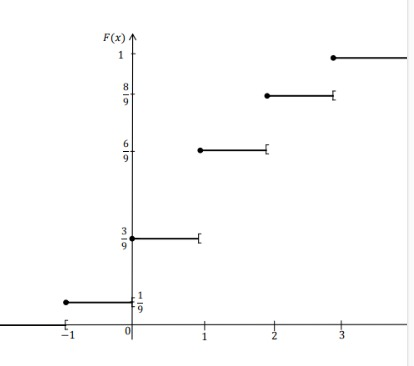
\includegraphics[width=0.5\textwidth]{/home/pathegobelba/Documents/LatexCodes/TS/build/repart.png} % Remplacez "nom_de_l_image.png" par le nom de votre fichier image
    \label{fig:image1}
\end{figure}

\begin{enumerate}
    \item $ F : \mathbb{R} \to [0 ; 1] \quad \text{définie par} \quad x \mapsto P(X \leq x), $
          étant une loi de probabilité définie sur un univers fini et non vide. Dans un repère orthogonal, la représentation graphique de $F$ est la suivante :
          \begin{enumerate}
              \item   Déterminer $\lim_{x \to -\infty} F(x)$ et $\lim_{x \to +\infty} F(x)$.
              \item  Déterminer la loi de probabilité de $X$.
              \item Calculer les probabilités $P(X \leq 0)$ et $P(X \geq 1)$.
              \item Calculer l’espérance mathématique $E(X)$ et $X$.
              \item Vérifier que l’écart-type $\sigma(X)$ de $X$ est égal à $\frac{\sqrt{12}}{3}$.
          \end{enumerate}
    \item On dispose de deux urnes $U_1$ et $U_2$ contenant chacune 3 boules. Les boules de $U_1$ sont numérotées 1, 2 et 3 et celles de $U_2$ sont numérotées -2, -1 et 0. On tire simultanément une boule de chaque urne et on effectue la somme $Y$ des numéros des boules tirées.
          \begin{enumerate}
              \item  Dresser un tableau à double entrée permettant d’obtenir les valeurs possibles de $Y$.
              \item En déduire que $X$ et $Y$ ont la même loi de probabilité.
          \end{enumerate}
\end{enumerate}

\section*{\fbox{\textbf{\exo}}\quad BAC S2 2019}

Dans une classe de première S2, sur 45 élèves 30 ont eu la moyenne au premier devoir de mathématiques. On considère que dans cette classe si un élève a la moyenne à un devoir donné la probabilité qu’il ait la moyenne au devoir suivant est $ \frac{1}{2} $ et s’il a raté la moyenne à un devoir donné la probabilité qu’il ait la moyenne au devoir suivant est $ \frac{1}{3} $.

Soit $E_n$ l’événement « l’élève a eu la moyenne au $n^{\text{ième}}$ devoir », $\overline{E_n}$ l’événement « l’élève n’a pas eu la moyenne au $n^{\text{ième}}$ devoir » et $p_n$ la probabilité de l’événement $E_n$.

\begin{enumerate}
    \item Déterminer $p_1$.
    \item 
    \begin{enumerate}
        \item Déterminer $P(E_2 / E_1)$ et $P(E_2 / \overline{E_1})$.
        \item En déduire $p_2$.
    \end{enumerate}
    \item Montrer que pour tout entier naturel non nul $n$, on a : $p_{n+1} = \frac{1}{6}p_n + \frac{1}{3}.$
    \item Soit $(u_n)$ la suite définie pour tout entier naturel non nul, par : $u_n = p_n - \frac{2}{5}$.
    \begin{enumerate}
        \item Montrer que $(u_n)$ est une suite géométrique dont on précisera la raison et le premier terme.
        \item Exprimer $u_n$ en fonction de $n$ puis $p_n$ en fonction de $n$.
        \item Calculer la limite de $p_n$ quand $n$ tend vers l’infini.
    \end{enumerate}
\end{enumerate}

\section*{\fbox{\textbf{\exo}}\quad BAC S2 2020}

\begin{enumerate}
    \item On dispose de deux dés cubiques dont les faces sont numérotées de 1 à 6. On lance simultanément les deux dés et on s'intéresse à la somme $S$ des chiffres apparus sur la face de dessus.
    \begin{enumerate}
        \item Déterminer les valeurs possibles de $S$.
        \item Déterminer la probabilité d’obtenir une somme égale à 9.
    \end{enumerate}

    \item Marame et Birane disposent chacun de deux dés et s’adonnent au jeu précédent, chacun de son côté.
    \begin{enumerate}
        \item Quelle est la probabilité que chacun affiche un même score de 9, 7 ou 8 ?
        \item Quelle est la probabilité qu’ils affichent le même score ?
        \item Celui qui affiche le plus grand score gagne. Calculer la probabilité pour que Marame gagne.
    \end{enumerate}
\end{enumerate}

\section*{\fbox{\textbf{\exo}}\quad BAC S2 2021}

Une urne $U_1$ contient quatre boules noires et trois boules blanches. 
Une urne $U_2$ contient trois boules noires et deux boules blanches.

Expérience : on jette un dé à 6 faces numérotées de 1 à 6, chaque face ayant la même probabilité d'apparaître. Si la face numérotée 6 apparaît, on tire une boule de $U_1$ sinon on tire une boule de $U_2$.
On considère les événements suivants : 
\begin{itemize}
    \item $A$ : « obtenir une face numérotée 6 ».
    \item $B$ : « tirer une boule blanche ».
\end{itemize}

\begin{enumerate}
    \item Schématiser la situation de l’expérience sous forme d’un arbre pondéré.
    \item Déterminer les probabilités de $A$ et $\overline{A}$, où $\overline{A}$ est l’événement contraire de $A$.
    \item Déterminer la probabilité de l’événement $B$.
    \item Déterminer $P_B(A)$, la probabilité de $A$ sachant $B$.
    \item L’expérience précédente se déroule 5 fois de suite de façon indépendante. Soit $X$ la variable aléatoire égale au nombre de boules blanches obtenues.
    \begin{enumerate}
        \item Déterminer la loi de probabilité de $X$.
        \item Trouver l’espérance mathématique de $X$, $E(X)$ et la variance de $X$, $V(X)$.
    \end{enumerate}
    \item L’expérience se déroule en $n$ parties indépendantes. Déterminer la valeur minimale de $n$ pour laquelle la probabilité d’obtenir au moins une boule blanche dépasse 0,99.
\end{enumerate}

\section*{\fbox{\textbf{Exercice 9}}\quad BAC S2 2022}
On jette trois fois de suite un dé non truqué à six faces portant les chiffres allant de 1 à 6. On lit les numéros des faces supérieures et on les note dans l'ordre $a$, $b$ et $c$. Puis on forme l’équation du second degré $(E) : ax^2 + bx + c = 0$. On note $\Omega$ l’univers de cette expérience aléatoire.

\begin{enumerate}
    \item Soit $A$ « $-1$ est solution de $(E)$ et $b = 6$ ». Justifier que la probabilité de l’événement $A$ est $p(A) = \frac{5}{216}$.
    \item On considère les événements suivants :
    \begin{itemize}
        \item $B$ : « $-2$ est solution de $(E)$ et $c = 4$ ».
        \item $C$ : « la somme des solutions est $-2$ et leur produit est $1$ ».
        \item $D$ : « les deux solutions sont confondues et $b = 4$ ».
    \end{itemize}
    La probabilité de chacun des événements $B$, $C$ et $D$ appartient à l’intervalle $I = \left\{ \frac{1}{72}, \frac{1}{108}, \frac{1}{54} \right\}$. Donner la probabilité de chacun des événements $B$, $C$ et $D$ en le justifiant.
    \item L’épreuve précédente est répétée 10 fois de suite et de façon indépendante. 
    \begin{enumerate}
        \item Soit $F$ l’événement : « L’événement $A$ se réalise une seule fois au $3^{\text{ème}}$ essai ». Montrer que la probabilité de l’événement $F$ est $p(F) = \frac{5 \times (211)^9}{(216)^{10}}$. 
        \item Soit $Y$ la variable aléatoire égale au nombre de réalisations de l’événement $A$ à l’issue des 10 épreuves. 
        \begin{enumerate}
            \item Déterminer la loi de probabilité de $Y$.
            \item Montrer que le nombre espéré de réalisations de $A$ est égal à $\frac{25}{108}$.
            \item Calculer la variance de $Y$.
        \end{enumerate}
    \end{enumerate}
\end{enumerate}
\end{document}